\label{chapter:metodo}
Este capítulo apresenta as etapas do método proposto para o funcionamento do sistema computacional da luva Hand.io e está explicado como os objetivos deste trabalho serão satisfeitos. 

\section{Visão geral do método da Hand.io}

A Hand.io é uma luva de controle que permite que quem a use realize gestos para controlar os dispositivos eletrônicos disponíveis em um dado ambiente. O projeto conta com uma luva de pano com um dispositivo preso ao tecido, que lê os movimentos da mão do usuário e uma central de processamento posicionada em um local estratégico, que recebe os sinais dos gestos através de uma conexão sem fio e executa as ações previamente definidas correspondentes a eles, conforme \autoref{fig:bigpicture}.

\begin{figure}[ht]
    \centering
    \caption{Visão geral do protótipo.}
    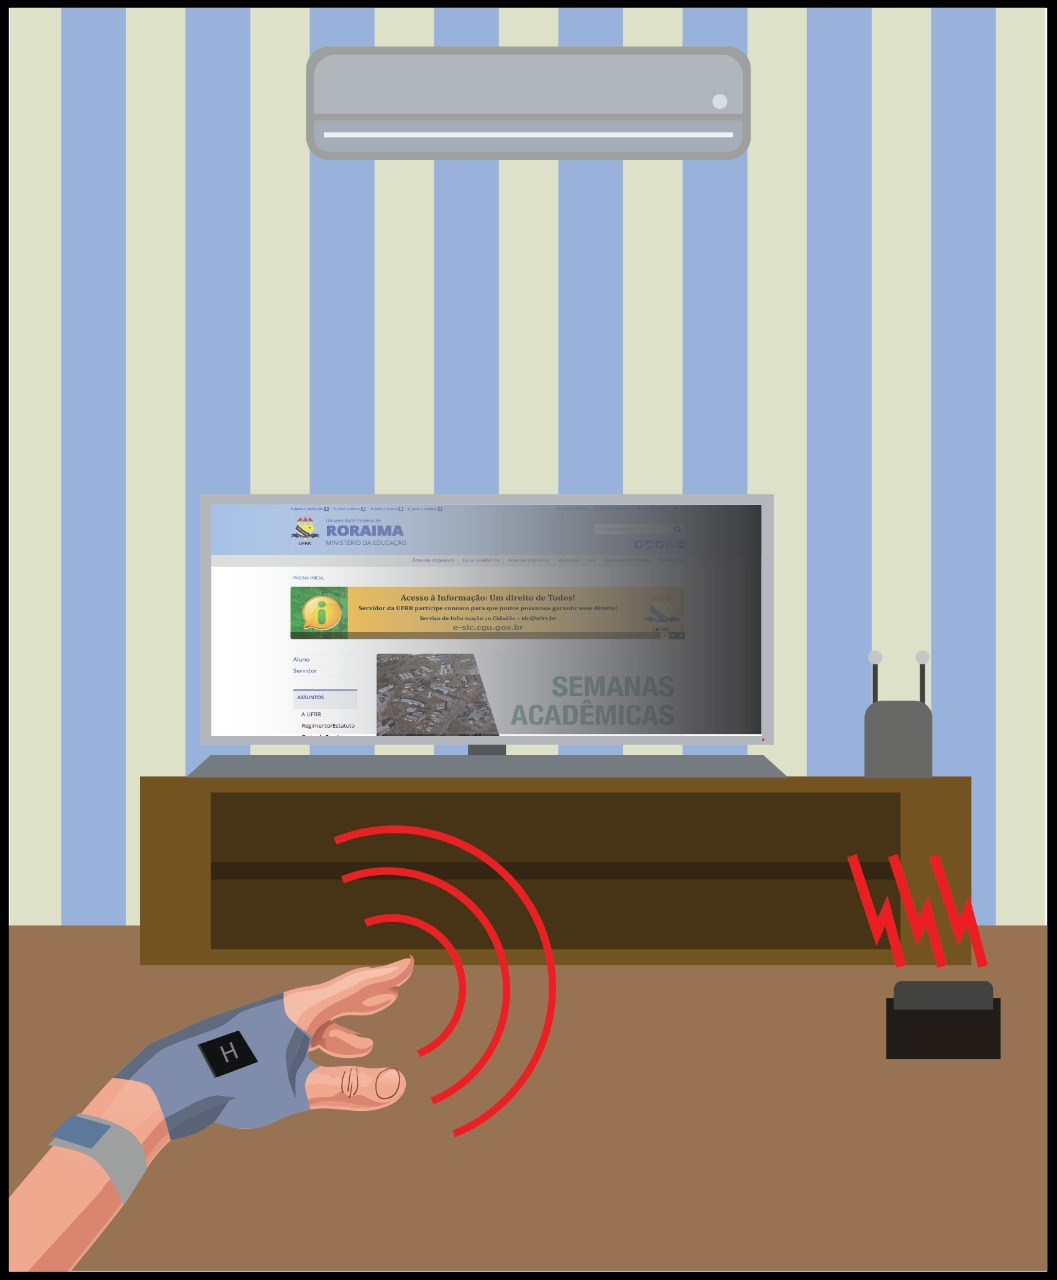
\includegraphics[width=0.5\textwidth, keepaspectratio]{resources/bigpicture.jpeg}
    \legend{Fonte: Elaborada pelo autor.}
    \label{fig:bigpicture}
\end{figure}

Os sinais dos movimentos são processados pela central utilizando algoritmos de aprendizado de máquina, que classificam o gesto realizado e realizam as ações correspondentes que estão definidas no banco de dados do sistema.

%Após os gestos terem sido reconhecidos com sucesso, a central de controle realiza a ação que 

\section{Fluxo de execução da Hand.io}

A~\autoref{fig:fluxograma}, descreve o método proposto para a luva Hand.io através de um fluxograma, mostrando as diferentes etapas de funcionamento da luva de maneira sequencial. Os itens do fluxograma apresentado abaixo significam:
% 
\begin{itemize}
    \item A posição inicial do fluxograma é definida por uma \textbf{seta sem origem} a partir da qual são realizadas as checagens iniciais do sistema.
    \item Os \textbf{losangos} representam condições onde dependendo do resultado o fluxo do sistema pode ser alterado, no primeiro momento é verificada a conexão com a luva de controle e logo depois o sistema verifica se existem dispositivos cadastrados, caso não existam o sistema aguarda pela inserção de dispositivos no banco de dados.
    \item Os \textbf{trapézios} representam ações externas que são realizadas pelo usuário, seja a partir da luva ou a partir do dispositivo que será utilizado para realizar o cadastro de novos dispositivos. 
    \item \textbf{Retângulos} representam processos internos do sistema 
e quadrados com barras laterais representam os processos predefinidos do sistema.
    \item O banco de dados que armazena os dados de gestos e códigos de infra-vermelhos de controle de dispositivos, está representado por um \textbf{cilindro} encontrado na parte central da figura.
\end{itemize}


\begin{figure}[ht]
    \centering
    \caption{Fluxograma da Hand.io.}
	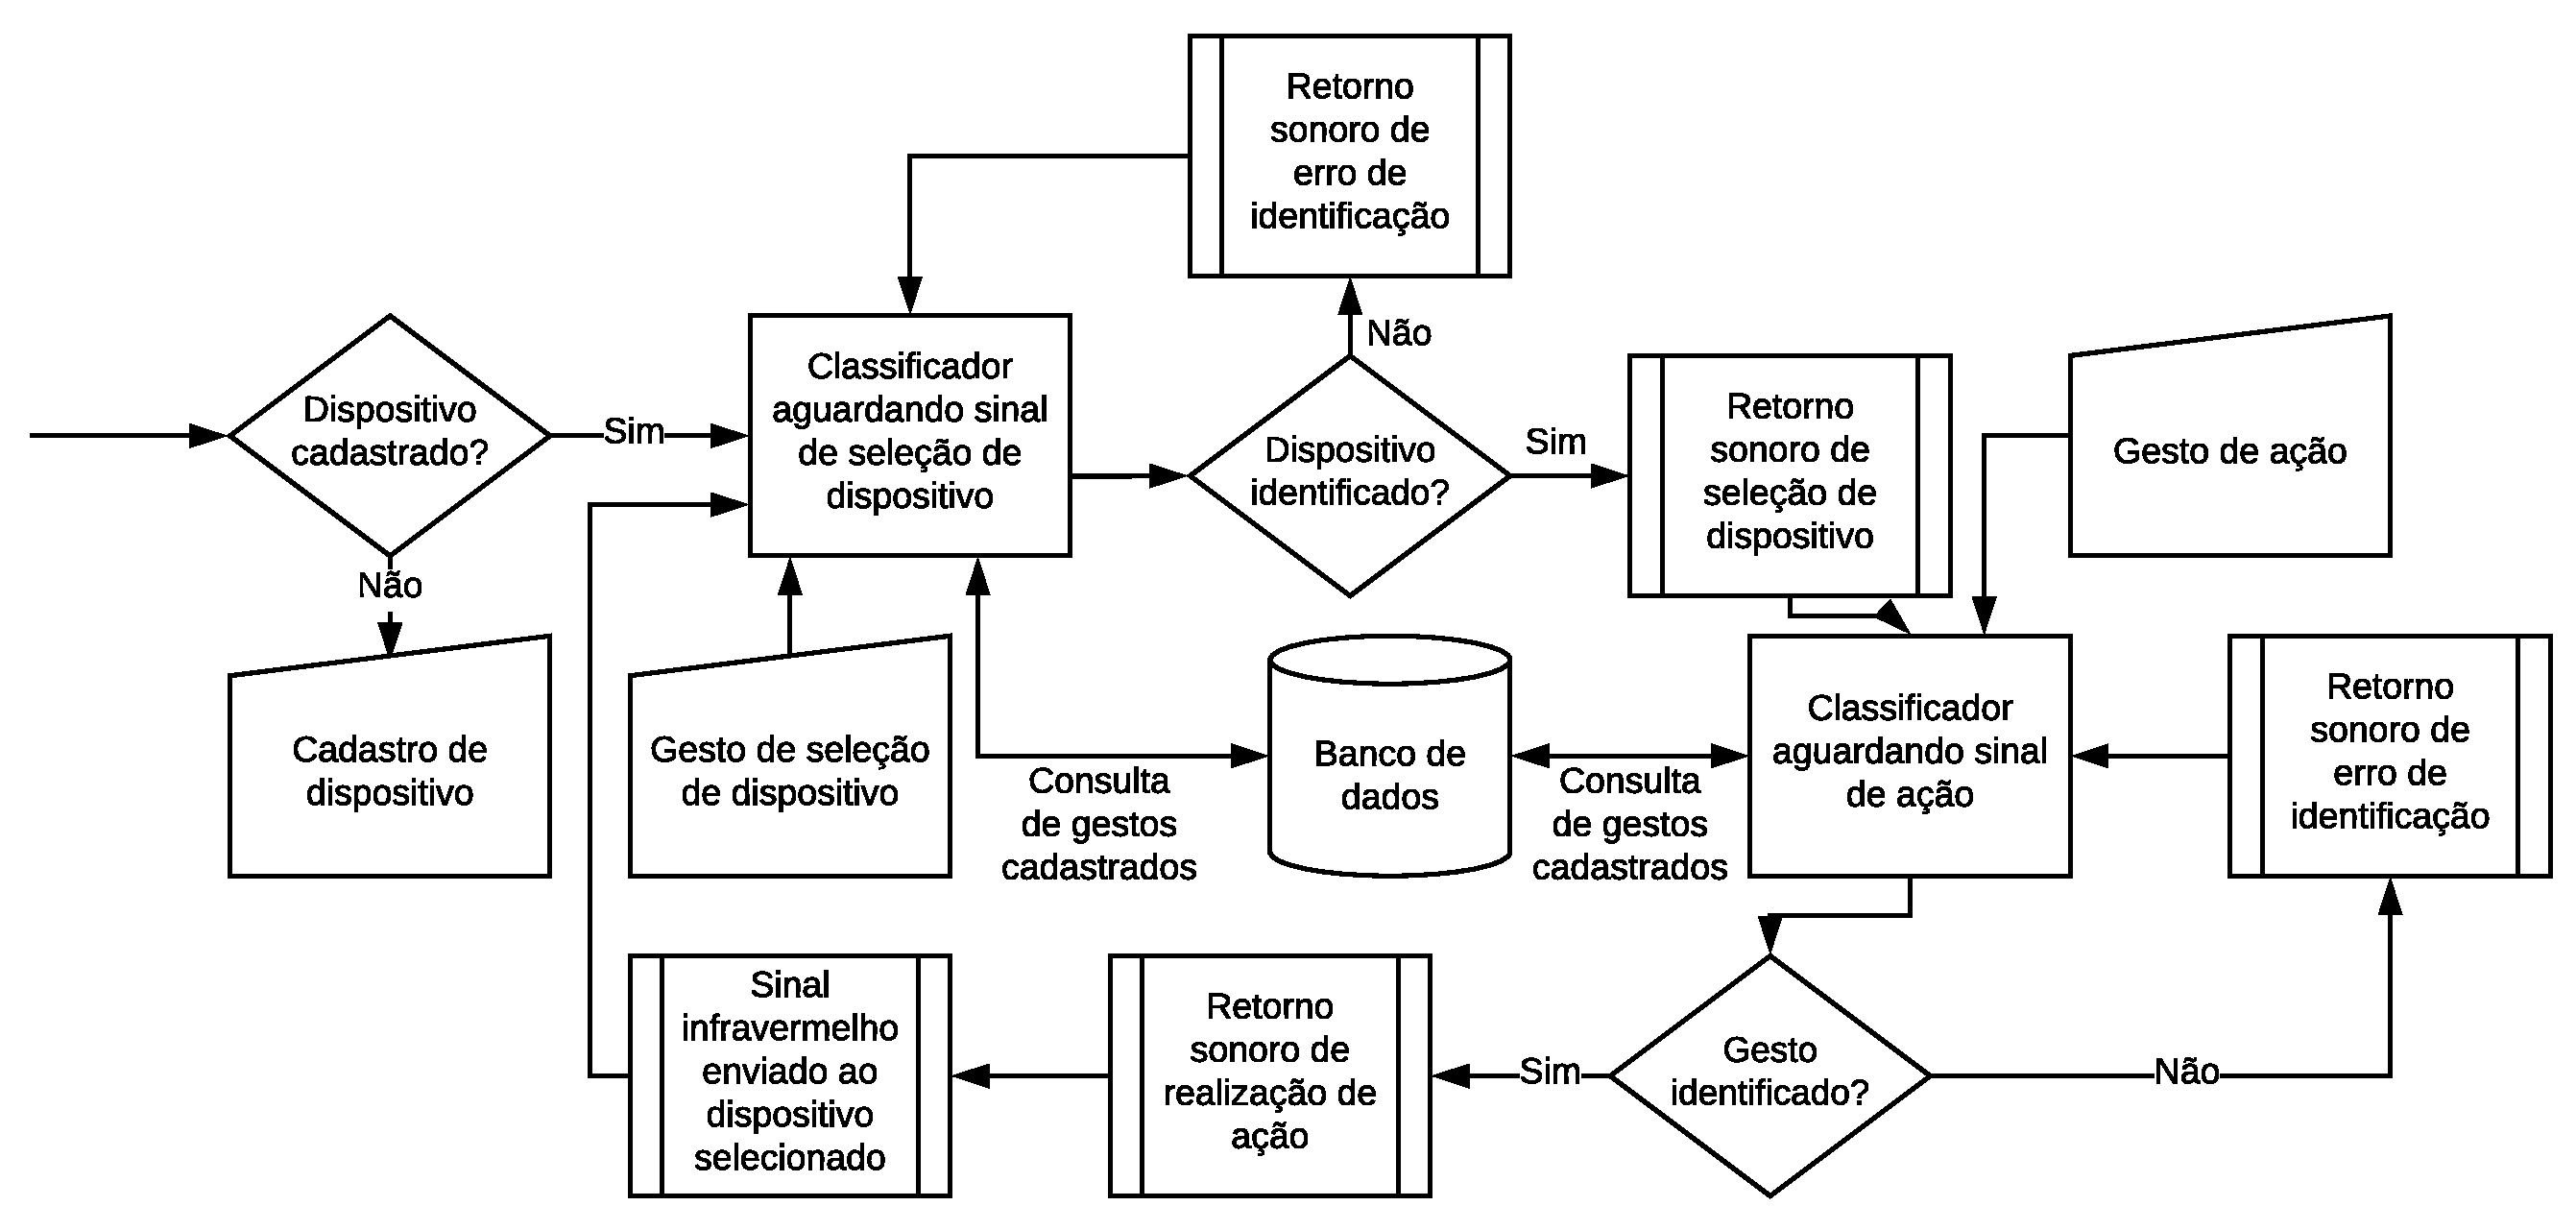
\includegraphics[width=\textwidth, keepaspectratio]{resources/fluxograma.pdf}
	\legend{Fonte: Elaborada pelo autor.}
	\label{fig:fluxograma}
\end{figure}




\section{Captura de Dados Baseado em Movimentos de Amplitude de Punho e Mão}

A ideia principal da luva Hand.io é que o usuário controle seu ambiente utilizando gestos da maneira mais natural possível, para isso os movimentos do usuário são capturados constantemente e enviados para a central em tempo real até que seja identificado um gesto correspondente a um dispositivo cadastrado, como pode ser observado na~\autoref{fig:fluxograma}.

A luva Hand.io utiliza dois sensores para realizar a captura dos movimentos da mão do usuário, um acelerômetro e um giroscópio. Estes dois sensores foram escolhidos visando evitar problemas encontrados no trabalho de \citeonline{uwave:2009}, exposto na Seção~\ref{cor:uwave}, que sofre problemas de precisão devido a presença de apenas um sensor acelerômetro.
% 
Os sensores escolhidos realizam diversas amostras nas mudanças na aceleração e no giro realizados na luva, que serão enviados em tempo real à central de processamento.%\todo{Apresentar exemplos de dados gerados pelos sensores}. 



\subsection{Conexão com a central de processamento}

A central de processamento (semelhante ao um pequeno aparelho de TV a cabo) inicia a sua operação esperando o recebimento de algum sinal da luva e até que a conexão tenha sido confirmada.
% , não realiza qualquer ação
% 
A conexão entre a luva e a central é realizada utilizando o protocolo de redes sem fio IEEE $802$.$11$~\cite{802.11:1997}, conhecida popularmente como Wi-Fi, através de uma rede LAN. Este protocolo foi escolhido por ter uma boa relação custo benefício de implementação levando também em consideração velocidade de transmissão de dados e alcance. A necessidade de permitir que o usuário se movimente livremente em um ambiente requer que a conexão sem fio tenha um alcance amplo.
%\todo{Descrever pq este protocolo foi escolhido, suas vantagens}. 

% Os sinais 

\section{Reconhecimento de Padrões Baseado em Movimentos e Ações}

Os sinais recebidos pela central de processamento servem de entrada para algoritmos de aprendizado de máquina, como ocorre no trabalho de \citeonline{uwave:2009} encontrado na Seção~\ref{cor:uwave}, que ficam em constante execução tentando classificar os sinais recebidos em categorias previamente escolhidas pelo desenvolvedor do sistema. 

%\todo{Apresentar ferramentas que pretende usar com Machine Learning}. 

Os possíveis gestos reconhecidos pela luva estão definidos durante a fase de implementação e contaram com a ajuda de um grupo de voluntários que serviram de referência para o desenvolvimento de gestos simples e coesos, como os apresentados na \autoref{fig:gestos}. O trabalho de \citeonline{imhome:2011} encontrado na Seção~\ref{cor:home} demonstra que um grande grupo de voluntários é fundamental para a criação de um vocabulário de gestos eficiente.

\begin{figure}[ht]
    \centering
    \caption{Exemplos de gestos.}
    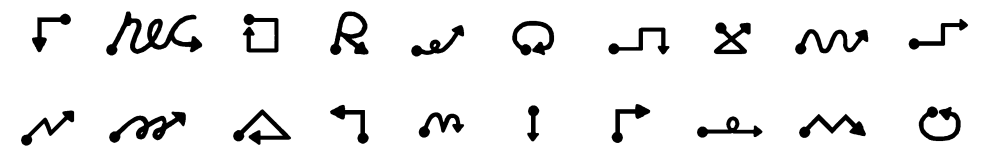
\includegraphics[width=0.6\textwidth, keepaspectratio]{resources/gestos.png}
    \legend{Fonte: \citeonline{accelerometer:2006}.}
    \label{fig:gestos}
\end{figure}

%\todo{Apresentar um figura com possíveis gestos para mostrar a vantagem de usar uma luva}. 

Gestos pré definidos e gestos criados pelos usuários são a abordagem mais efetiva para controlar um ambiente.
No entanto uma quantidade muito grande de gestos, e movimentos muito complexos não são a melhor escolha, pois existem uma quantidade limitada de gestos que podem ser lembrados com precisão sem que haja confusão durante a realização de um determinado gesto.

Neste método foi desenvolvido um extensivo \textit{training set} com dados recolhidos de voluntários realizando os gestos. Estes dados são utilizados como modelo de treinamento para algoritmos de aprendizado de máquina, como os apresentados por \cite{uwave:2009} na Seção~\ref{cor:uwave}, que irão reconhecer os gestos realizados pelo usuário. Foi utilizado o \textit{framework} \textit{Python} Scikit-learn \cite{scikit-learn}, levando em consideração o tamanho do \textit{training set} e a capacidade computacional da central de processamento. 

Existem dois momentos durante o fluxo de execução da Hand.io onde estes algoritmos são utilizados, quando o sistema aguarda que o usuário selecione o dispositivo que ele deseja controlar e quando o sistema aguarda um comando que será realizado no dispositivo selecionado, ambos os momentos podem ser vistos respectivamente na \autoref{fig:fluxograma} na letra B. A cada vez que os algoritmos finalizam a classificação dos sinais tidos como entrada, o sistema retorna para o usuário um sinal sonoro de confirmação. 




\section{Modelo de Conexão Entre Dispositivos Eletrônicos}

O controle dos dispositivos se dá utilizando um LED infravermelho, seguindo um padrão de controle remoto bem estabelecido pela industria de eletrônicos de consumo. Cada fabricante define um protocolo de códigos infravermelhos específicos para cada dispositivo como o protocolo SIRC que é utilizado pela Sony em suas TVs \cite{sirc} e o protocolo RC5 que é utilizado pela Philips \cite{rc5}. Protocolos diferentes foram criados visando impedir a interferência entre controles e dispositivos de fabricantes diferentes, como por exemplo o usuário tentar ligar o ar condicionado e acabar ligando a TV por acidente.

Os códigos de controle remoto de cada dispositivo cadastrado no sistema ficam armazenados em um banco de dados localizado na central de processamento. Cada código estará relacionado à um gesto específico que quando classificado pelo sistema será executado. Durante o cadastro de dispositivos, exibido na \autoref{fig:fluxograma} letra A, o sistema pede ao usuário que pressione os botões do controle remoto do dispositivo a ser controlado correspondentes às ações que ele deseja realizar por gestos. A intenção é que a base de dados dos sinais de infravermelho seja populada ao ponto de que sejam criados perfis pré definidos para cada dispositivo, para que quando um dispositivo já presente na base de dados seja cadastrado, não seja necessário realizar o cadastro dos sinais manualmente. 

%\section{Inferência de Comportamentos para Acionamento de Dispositivos Eletrotônicos}

%Com o passar do uso da luva 

\section{Modelo de Prototipação}

Os componentes utilizados para a confecção do protótipo da luva e da central buscam ter o menor custo possível, sem comprometer os recursos computacionais necessários para o funcionamento nominal do sistema, uma relação de preços do projeto pode ser vista na \autoref{tab:custos}. 

%Componentes produzidos em massa que já tem sua utilização testada extensivamente pela comunidade foram selecionados\todo{Apresentar exemplos}. 

\begin{table}[ht]
    \centering
    \caption{Estimativa de preços dos componentes.}
    \begin{tabular}{|l|c|}
        \hline
        \textbf{Componentes}   & \textbf{Preços}   \\ \hline
        Raspberry pi 3         & R\$ 239,90        \\ \hline
        Sensor MPU-6050        & R\$ 23,90         \\ \hline
        Módulo WiFi ESP8266-01 & R\$ 26,90         \\ \hline
        Receptor Infravermelho TSOP4838 & R\$ 6,90 \\ \hline
        LED Emissor Infravermelho       & R\$ 0,90 \\ \hline
        \textbf{Total}         & R\$ 298,50        \\ \hline
    \end{tabular}
    \legend{Fonte: \citeonline{filipeflop}.}
    \label{tab:custos}
\end{table}

O protótipo é composto pela luva em si que conta com sensores que irão capturar os movimentos do usuário apresentado na \autoref{fig:esq_luva}, e pela central de processamento que irá realizar as ações correspondentes aos gestos exibida na \autoref{fig:esq_central}, nos dispositivos conectados.

%\todo[inline]{Descrever quais são os componentes da central}

A luva conta uma placa GY-$521$ que tem um sensor MPU-$6050$~\cite{invensense}, apresentado no canto direito da \autoref{fig:esq_luva}. Esta placa é utilizada em diversos projetos que utilizam captura de movimentos devido a sua boa relação custo benefício em relação a precisão dos sensores. O sensor MPU-$6050$~\cite{invensense} conta com um acelerômetro e um giroscópio de três eixos cada, e um processador de sinais digitais integrado que pode ser utilizado para pré processar os sinais da luva antes que eles sejam enviados para a central de processamento, reduzindo a carga de trabalho realizada pela central.

A comunicação com a central de processamento ocorre utilizando uma placa Wi-Fi ESP-$8266$, segundo componente da direita para a esquerda na \autoref{fig:esq_luva}, que pode enviar sinais de maneira independente à qualquer computador conectado a uma rede LAN. Como fonte de energia a luva irá utilizar um conjunto de baterias que terão sua voltagem ajustada por um regulador, já que tanto a placa GY-521 quanto a placa Wi-Fi ESP-$8266$ podem funcionar com uma voltagem nominal de 3.3v.



%\todo[inline]{Descrever as figuras apresentadas abaixo, e razão da escolho do arduino.}

\begin{figure}[ht]
    \centering
    \caption{Esquemático do protótipo da luva.}
    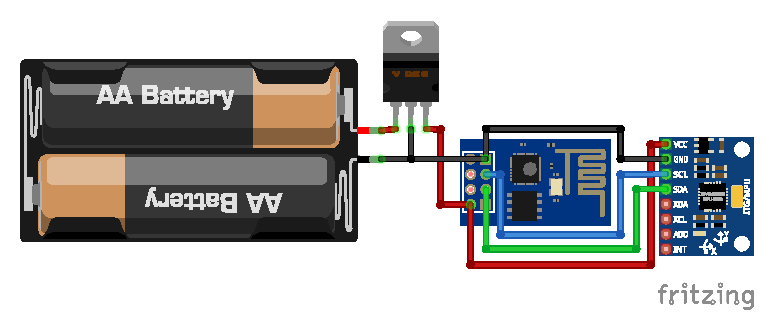
\includegraphics{resources/esquematico_tcc_bb.pdf}
    \legend{Fonte: Elaborada pelo autor.}
    \label{fig:esq_luva}
\end{figure}

Os componentes da central de processamento, apresentados na \autoref{fig:esq_central}, são compostos por um Raspberry Pi 3 \cite{raspberry:pi3} que ficará conectado à internet esperando os sinais da luva e realizará o reconhecimento dos sinais, um receptor infravermelho TSOP4838 que serve para a realização do cadastro de novos dispositivos e um LED emissor de sinais infravermelhos que podem ser reconhecidos por dispositivo que utilizam este protocolo como meio de controle.

\begin{figure}[ht]
    \centering
    \caption{Esquemático da central de processamento de sinais e execução de ações.}
    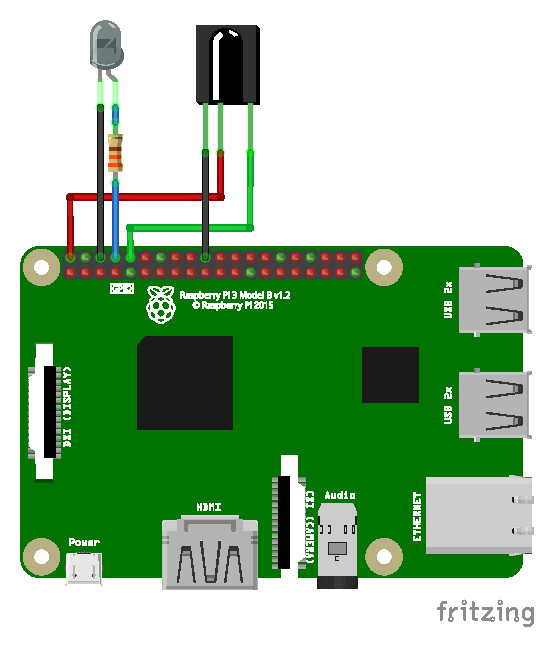
\includegraphics[width=0.55\textwidth, keepaspectratio]{resources/esquematico_central_bb.pdf}
    \legend{Fonte: Elaborada pelo autor.}
    \label{fig:esq_central}
\end{figure}

O Raspberry Pi 3 \cite{raspberry:pi3} foi escolhido devido ao seu tamanho compacto e sua alta capacidade de processamento. Por se tratar de um computador completo em uma placa é possível instalar uma distribuição de Linux com capacidade de se conectar à internet com certa facilidade. Graças à sua unidade de processamento gráfico (GPU, em inglês) integrada, o Raspberry Pi 3 consegue executar algoritmos de aprendizado de máquina de maneira eficaz, frameworks como o TensorFlow conseguem tirar todo proveito destes componentes através de paralelismo.

% \section{Modelagem da Hand.io}
% 
% Durante a fase de modelagem do sistema, serão desenvolvidos diagramas utilizando UML que servirão de guia para a implementação do protótipo da Hand.io. Será desenvolvida também, uma máquina de estados que irá modelar o comportamento do sistema de maneira, levando em consideração que a luva e a central de processamento de sinais funcionam de maneira independente uma da outra, se faz necessário este tipo de modelagem para reduzir a imprevisibilidade do sistema. 

%Graças à natureza formal dos diagramas UML, é possível realizar testes e verificações automatizadas a partir deles em ferramentas como o FOREVER \cite{forever}.

%\todo[inline]{Se tiver o diagram de sequência sugiro adicionar.}


%A rede de Petri será testada extensivamente utilizando ferramentas de verificação automatizadas, para detectar se ocorrerão problemas como os citados por \citeonline{peterson:1981} na Seção~\ref{def:petri_prop}.

%\todo[inline]{Falta descrever onde os modelos formais serão usados para garantir a qualidade do produto}

